% vim: set spell spelllang=en tw=100 et sw=4 sts=4 foldmethod=marker foldmarker={{{,}}} :

\documentclass{beamer}

\usepackage{tikz}
\usepackage{xcolor}
\usepackage{complexity}
\usepackage{hyperref}
\usepackage{microtype}
\usepackage{amsmath}                   % \operatorname
\usepackage{amsfonts}                  % \mathcal
\usepackage{amssymb}                   % \nexists
\usepackage{gnuplot-lua-tikz}          % graphs
\usepackage[vlined]{algorithm2e} % algorithms

\usetikzlibrary{shapes, arrows, shadows, calc, positioning, fit}
\usetikzlibrary{decorations.pathreplacing, decorations.pathmorphing, shapes.misc}
\usetikzlibrary{tikzmark}

\definecolor{uofguniversityblue}{rgb}{0, 0.219608, 0.396078}
\colorlet{uofguniversityblue40}{uofguniversityblue!40!white}

\definecolor{uofgheather}{rgb}{0.356863, 0.32549, 0.490196}
\definecolor{uofgaquamarine}{rgb}{0.603922, 0.72549, 0.678431}
\definecolor{uofgslate}{rgb}{0.309804, 0.34902, 0.380392}
\definecolor{uofgrose}{rgb}{0.823529, 0.470588, 0.709804}
\definecolor{uofgmocha}{rgb}{0.709804, 0.564706, 0.47451}

\definecolor{uofglawn}{rgb}{0.517647, 0.741176, 0}
\definecolor{uofgcobalt}{rgb}{0, 0.615686, 0.92549}
\definecolor{uofgturquoise}{rgb}{0, 0.709804, 0.819608}
\definecolor{uofgsunshine}{rgb}{1.0, 0.862745, 0.211765}
\definecolor{uofgpumpkin}{rgb}{1.0, 0.72549, 0.282353}
\definecolor{uofgthistle}{rgb}{0.584314, 0.070588, 0.447059}
\definecolor{uofgpillarbox}{rgb}{0.701961, 0.047059, 0}
\definecolor{uofglavendar}{rgb}{0.356863, 0.301961, 0.580392}

% {{{ theme things
\useoutertheme[footline=authortitle]{miniframes}
\useinnertheme{rectangles}

\setbeamerfont{block title}{size={}}
\setbeamercolor*{structure}{fg=uofguniversityblue}
\setbeamercolor*{palette primary}{use=structure,fg=black,bg=white}
\setbeamercolor*{palette secondary}{use=structure,fg=black,bg=uofguniversityblue40}
\setbeamercolor*{palette tertiary}{use=structure,fg=white,bg=uofguniversityblue}
\setbeamercolor*{palette quaternary}{fg=white,bg=black}

\setbeamercolor*{titlelike}{parent=palette primary}

\beamertemplatenavigationsymbolsempty

\setbeamertemplate{title page}
{
    \begin{tikzpicture}[remember picture, overlay]
        \node [anchor=center, fill=white, fill opacity=0.8, text opacity=1, inner sep=0.2cm, shift={(0cm,0.3cm)}] at (current page.center) {
            \begin{minipage}{\paperwidth}
                \centering
                {\usebeamerfont{title}\inserttitle}
                \vskip0.2cm
                {\usebeamerfont{author}\insertauthor \quad \insertinstitute}
            \end{minipage}
        };
    \end{tikzpicture}

    \begin{tikzpicture}[remember picture, overlay]
        \node at (current page.north west) {\begin{tikzpicture}[remember picture, overlay]\fill
        [fill=uofguniversityblue, anchor=north west] (0, 0) rectangle (\paperwidth, -1.5cm);\end{tikzpicture}};
        \node [anchor=north west, shift={(0.2cm,-0.2cm)}] at (current page.north west) {\includegraphics*[keepaspectratio=true,scale=0.5]{UoG_keyline.pdf}};
    \end{tikzpicture}
}

\setbeamertemplate{section page}
{
    \begin{centering}
        \begin{beamercolorbox}[sep=12pt,center]{part title}
            \usebeamerfont{section title}\insertsection\par
        end{beamercolorbox}
    \end{centering}
}

\newcommand{\frameofframes}{/}
\newcommand{\setframeofframes}[1]{\renewcommand{\frameofframes}{#1}}

\makeatletter
\setbeamertemplate{footline}
{%
    \begin{beamercolorbox}[colsep=1.5pt]{upper separation line foot}
    \end{beamercolorbox}
    \begin{beamercolorbox}[ht=2.5ex,dp=1.125ex,%
        leftskip=.3cm,rightskip=.3cm plus1fil]{author in head/foot}%
        \leavevmode{\usebeamerfont{author in head/foot}\insertshortauthor}%
        \hfill%
        {\usebeamerfont{institute in head/foot}\usebeamercolor[fg]{institute in head/foot}\insertshortinstitute}%
    \end{beamercolorbox}%
    \begin{beamercolorbox}[ht=2.5ex,dp=1.125ex,%
        leftskip=.3cm,rightskip=.3cm plus1fil]{title in head/foot}%
        {\usebeamerfont{title in head/foot}\insertshorttitle}%
        \hfill%
        {\usebeamerfont{frame number}\usebeamercolor[fg]{frame number}\insertframenumber~\frameofframes~\inserttotalframenumber}
    \end{beamercolorbox}%
    \begin{beamercolorbox}[colsep=1.5pt]{lower separation line foot}
    \end{beamercolorbox}
}

% }}}

\title{Parallel Search, Backjumping, and Brittle Skeletons}
\author{Ciaran McCreesh and Patrick Prosser}

\begin{document}

{
    \usebackgroundtemplate{
        \tikz[overlay, remember picture]
        \node[at=(current page.south), anchor=south, inner sep=0pt]{\includegraphics*[keepaspectratio=true, width=\paperwidth]{background.jpg}};
    }
    \begin{frame}[plain,noframenumbering]
        \titlepage
    \end{frame}
}

\begin{frame}{The Subgraph Isomorphism Problem}

    \centering
    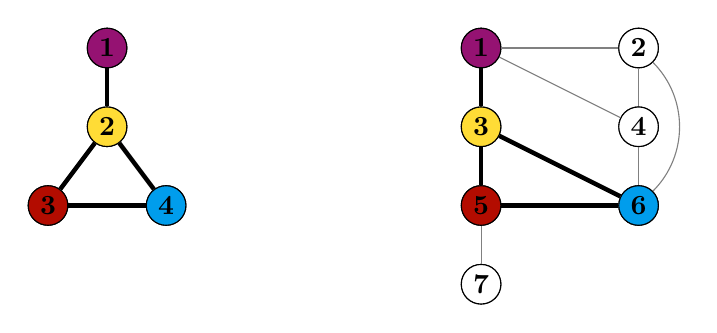
\begin{tikzpicture}%{{{
        \node <1> [draw, circle, fill=white, inner sep=2pt, font=\bfseries] (Na) at (0.75,  0) {1};
        \node <1> [draw, circle, fill=white, inner sep=2pt, font=\bfseries] (Nb) at (0.75, -1) {2};
        \node <1> [draw, circle, fill=white, inner sep=2pt, font=\bfseries] (Nc) at (0, -2) {3};
        \node <1> [draw, circle, fill=white, inner sep=2pt, font=\bfseries] (Nd) at (1.5, -2) {4};

        \node <2> [draw, circle, fill=uofgthistle, inner sep=2pt, font=\bfseries] (Na) at (0.75,  0) {1};
        \node <2> [draw, circle, fill=uofgsunshine, inner sep=2pt, font=\bfseries] (Nb) at (0.75, -1) {2};
        \node <2> [draw, circle, fill=uofgpillarbox, inner sep=2pt, font=\bfseries] (Nc) at (0, -2) {3};
        \node <2> [draw, circle, fill=uofgcobalt, inner sep=2pt, font=\bfseries] (Nd) at (1.5, -2) {4};

        \tikzstyle{edge} = [ultra thick];
        \tikzstyle{ledge} = [color = black!50!white];

        \draw <1> [ledge] (Na) -- (Nb);
        \draw <1> [ledge] (Nb) -- (Nc);
        \draw <1> [ledge] (Nc) -- (Nd);
        \draw <1> [ledge] (Nb) -- (Nd);

        \draw <2> [edge] (Na) -- (Nb);
        \draw <2> [edge] (Nb) -- (Nc);
        \draw <2> [edge] (Nc) -- (Nd);
        \draw <2> [edge] (Nb) -- (Nd);

        \node <1> [draw, circle, fill=white, inner sep=2pt, font=\bfseries] (N1) at (5.5,  0) {1};
        \node <1> [draw, circle, fill=white, inner sep=2pt, font=\bfseries] (N2) at (7.5,  0) {2};
        \node <1> [draw, circle, fill=white, inner sep=2pt, font=\bfseries] (N3) at (5.5, -1) {3};
        \node <1> [draw, circle, fill=white, inner sep=2pt, font=\bfseries] (N4) at (7.5, -1) {4};
        \node <1> [draw, circle, fill=white, inner sep=2pt, font=\bfseries] (N5) at (5.5, -2) {5};
        \node <1> [draw, circle, fill=white, inner sep=2pt, font=\bfseries] (N6) at (7.5, -2) {6};
        \node <1> [draw, circle, fill=white, inner sep=2pt, font=\bfseries] (N7) at (5.5, -3) {7};

        \node <2> [draw, circle, fill=uofgthistle, inner sep=2pt, font=\bfseries] (N1) at (5.5,  0) {1};
        \node <2> [draw, circle, fill=white, inner sep=2pt, font=\bfseries] (N2) at (7.5,  0) {2};
        \node <2> [draw, circle, fill=uofgsunshine, inner sep=2pt, font=\bfseries] (N3) at (5.5, -1) {3};
        \node <2> [draw, circle, fill=white, inner sep=2pt, font=\bfseries] (N4) at (7.5, -1) {4};
        \node <2> [draw, circle, fill=uofgpillarbox, inner sep=2pt, font=\bfseries] (N5) at (5.5, -2) {5};
        \node <2> [draw, circle, fill=uofgcobalt, inner sep=2pt, font=\bfseries] (N6) at (7.5, -2) {6};
        \node <2> [draw, circle, fill=white, inner sep=2pt, font=\bfseries] (N7) at (5.5, -3) {7};

        \draw [ledge] (N1) -- (N2);
        \draw [ledge] (N1) -- (N4);
        \draw [ledge] (N2) -- (N4);
        \draw [ledge] (N4) -- (N6);
        \draw [ledge] (N2) to [in=45, out=315] (N6);
        \draw [ledge] (N5) -- (N7);

        \draw <1> [ledge] (N1) -- (N3);
        \draw <1> [ledge] (N3) -- (N5);
        \draw <1> [ledge] (N3) -- (N6);
        \draw <1> [ledge] (N5) -- (N6);
        \draw <2> [edge] (N1) -- (N3);
        \draw <2> [edge] (N3) -- (N5);
        \draw <2> [edge] (N3) -- (N6);
        \draw <2> [edge] (N5) -- (N6);

    \end{tikzpicture}%}}}
    \\~

\end{frame}

\begin{frame}{Filtering}

\end{frame}

\begin{frame}{Backtracking Search}

\end{frame}

\begin{frame}{Search as a Tree}
\end{frame}

\begin{frame}{Work Stealing Matters}
\end{frame}

\begin{frame}{Preventing a Slowdown, Part 1}
\end{frame}

\begin{frame}{Backjumping}
\end{frame}

\begin{frame}{Backjumping as a Fold}
\end{frame}

\begin{frame}{Preventing a Slowdown, Part 2}
\end{frame}

\begin{frame}{Folding Zero}
\end{frame}

\begin{frame}{Preventing a Slowdown, Part 3}
\end{frame}

\begin{frame}{Some Grumpy Remarks about Brittle Skeletons}
\end{frame}

\begin{frame}{What's the Alternative?}

    \begin{itemize}
        \item <2-> Doing it by hand?
            \begin{itemize}
                \item This works, but is painful and error-prone\ldots
            \end{itemize}

        \item <3-> Better skeletons?
            \begin{itemize}
                \item But they would need to be very domain-specific, which defeats the point of
                    skeletons\ldots
            \end{itemize}

        \item <4-> External descriptions of search?
            \begin{itemize}
                \item I've yet to figure out why this will end up not being very good\ldots
            \end{itemize}
    \end{itemize}

\end{frame}

\begin{frame}[b]
    \begin{center}
    \url{http://dcs.gla.ac.uk/~ciaran} \\
    \href{mailto:c.mccreesh.1@research.gla.ac.uk}{\nolinkurl{c.mccreesh.1@research.gla.ac.uk}}
\end{center}
\begin{tikzpicture}[remember picture, overlay]
    \node at (current page.north west) {\begin{tikzpicture}[remember picture, overlay]\fill
    [fill=uofguniversityblue, anchor=north west] (0, 0) rectangle (\paperwidth, -1.5cm);\end{tikzpicture}};
    \node [anchor=north west, shift={(0.2cm,-0.2cm)}] at (current page.north west) {\includegraphics*[keepaspectratio=true,scale=0.5]{UoG_keyline.pdf}};
\end{tikzpicture}
\end{frame}

\end{document}

